\documentclass[
	ngerman,
	11pt,
	twoside,
	a4paper,
	headsepline,
	footsepline, 
	toc=bib
]{scrbook}
% \makeatletter
\DeclareOldFontCommand{\rm}{\normalfont\rmfamily}{\mathrm}
% \DeclareOldFontCommand{\sf}{\normalfont\sffamily}{\mathsf}
% \DeclareOldFontCommand{\tt}{\normalfont\ttfamily}{\mathtt}
\DeclareOldFontCommand{\bf}{\normalfont\bfseries}{\mathbf}
% \DeclareOldFontCommand{\it}{\normalfont\itshape}{\mathit}
% \DeclareOldFontCommand{\sl}{\normalfont\slshape}{\@nomath\sl}
\DeclareOldFontCommand{\sc}{\normalfont\scshape}{\@nomath\sc}


%!TEX root = thesis.tex
% \KOMAoption{toc}{listof,bib,idx}

%------------------------------------------------------------------------------
%- PAKETE
%------------------------------------------------------------------------------
	%DIN A4
		\usepackage{a4}

	%Direkte Eingabe von Umlauten mit Angabe von Schriftsatz
	%in Kombination mit 'german' sind jetzt ä direkt erlaubt!
		\usepackage[T1]{fontenc}
		%\usepackage[latin1]{inputenc}
		\usepackage[utf8]{inputenc}

	%Sprache einstellen (Inhaltsverzeichnis, ...)
		\usepackage[ngerman]{babel} %american,italian,german,english


	%Euro Zeichen
		\usepackage{eurosym}

	% Vereinfachtes Eingeben von Leerschlägen hinter Shortcut-Commands
	% Beispiel: \newcommand{\DNA}{desoxyribose nucleid acid\xspace}
		\usepackage{xspace}

	%Sortierte Literaturverweise
		%\usepackage{cite}

	% Kommentare
		\usepackage{verbatim}

	%Verbessertes Beschriften mir div. Optionen
		\usepackage{caption}

	%Zusaetzliche Symbole und Schriften (ams: american mathematical soc)
		\usepackage{amssymb}
		%\usepackage{amstext		%\usepackage{amsfonts}
		%\usepackage{amsbsy}
		%\usepackage{amscd}
		%\usepackage{latexsym}

	%Text Companion fonts which provide many text symbols (such as baht, bullet, copyright, musicalnote, onequarter, section, and yen) in the TS1 encoding.
		\usepackage{textcomp}

	%Drehen von Text, Tabellen, Seiten
		%\usepackage{rotating}

	%Schöne professionelle Tabellen mit
		\usepackage{booktabs}
		\usepackage{array}
		\usepackage{tabularx}
		\usepackage{tabulary}
		\usepackage{multirow}

	%including graphics files, rotating parts of a page, and scaling parts of a page
		\usepackage{graphicx}

	%Nice drawing package
		%\usepackage{tikz}

	%besserer eps import: \eps import ERSETZEN durch \epsfig
		\usepackage{epsf}

	%Farbunterstützung (ausserhalb der Bilder)
		\usepackage{xcolor}
		\definecolor{gray}{gray}{.75}
		\definecolor{colorUzLgreen}{RGB}{0,75,90} 
		\definecolor{colorUzLred}{RGB}{228,32,50}
		\definecolor{colorUzLblue}{RGB}{0,106,163}
		\definecolor{colorUzLgray}{RGB}{208,208,208}

	% Ändern der Ränder für das Titelblatt
		\usepackage[]{geometry} % showframe

	%Postcript einbinden, wobei Text ersetzt werden kann
		%\usepackage{psfrag}

	%Für den Index
		\usepackage{makeidx}
		\makeindex %Muss vor begin{document}, sonst passiert nix

	%Erleichterungen fürs Deutsche inkl Silbentrennung
		%\usepackage{german}

	%Ensure minimal spacing of table cells (http://www.ctan.org/tex-archive/help/Catalogue/entries/cellspace.html)
		%\usepackage{cellspace}

	%Source code Listings
		\usepackage{listings}

	%Subfigures
		\usepackage{subfigure}

	% Ignore float add to list warning
	\usepackage{scrhack}

	%Automatically adds the bibliography and/or the index and/or the contents, etc., to the Table of Contents listing.
		%\usepackage[nottoc]{tocbibind} %,notlot,notlof

	%Add Bibliography Packages
		\usepackage[
  		style=ACM-Reference-Format,
  		backend=biber,
  		sortcites=true,
  		maxbibnames=99,
  		defernumbers=true
		]{biblatex}
		\usepackage{csquotes}

	%St Mary Road symbols for theoretical computer science.
		%\usepackage{stmaryrd}

	%URL Darstellung
		\usepackage{url}

	%PDF und Standard Latex Unterscheidung
		\usepackage{ifpdf}

	%Abkürzungsverzeichnis
		\usepackage[intoc]{nomencl}
		  \let\abbrev\nomenclature
		  \renewcommand{\nomname}{Abkürzungsverzeichnis}
		  \setlength{\nomlabelwidth}{.25\hsize}
		  \renewcommand{\nomlabel}[1]{#1 \dotfill}
		  \setlength{\nomitemsep}{-\parsep}
		  \makenomenclature

	  \newcommand{\abk}[2]{#1\abbrev{#1}{#2}}

	%With \usepackage{ulem}, you have the following new commands:
		%    * \uline{important} underlined text
		%    * \uuline{urgent} double-underlined text
		%    * \uwave{boat} wavy underline
		%    * \sout{wrong} line drawn through word
		%    * \xout{removed} marked over with //////.
		%    * {\em phasized\/} and \emph{asized} In LaTeX, by default, these are underlined; use \normalem or [normalem] to restore italics
		%    * \useunder{\uwave}{\bfseries}{\textbf} use wavy underline in place of bold face
		%Note that this package changes \em and \emph to be underline. To change this behavior back to normal, use the \normalem command, for example
		%\usepackage{ulem}
		%\normalem
		%\usepackage[normalem]{ulem}

	  %\newcommand{\markup}[1]{\uline{#1}}

	% package to customize the three basic lists (enumerate, itemize and description)
	% by means of a set of parameters, and to clone them to define new "logical" lists.
		\usepackage{enumitem}
		\setitemize{enumsep=-3pt}
		\setitemize{itemsep=-3pt}

	%Definitionen
		\usepackage{theorem}
		\newcounter{theorem}
		\newtheorem{definition}[theorem]{Definition}


	\usepackage[bookmarks=true,
					bookmarksopen=true,
   					% Lesezeichen ausgeklappt
					bookmarksnumbered=true,
					colorlinks=true,
				   	%Einfärbung von Links
					linkcolor=black
					% Linkfarbe: schwarz
					]
				    % Anzeige der Kapitelzahlen am Anfang der Namen der Lesezeichen
				   {hyperref}

	
	% Todos
		% Alle Todos und Liste aller Todos zeigen
		\usepackage[colorinlistoftodos]{todonotes}
		% Alle Todos und Liste aller Todos deaktivieren
		%\usepackage[disable]{todonotes}

	%Darstellung von Algorithmen
	\usepackage{algorithm}
	\usepackage{algorithmic}

	%Zitate
		\newcounter{quotectr}
		\newtheorem{myquote}[quotectr]{Zitat}

%------------------------------------------------------------------------------
%- Layout
%------------------------------------------------------------------------------

	%Tiefe des Inhaltsverzeichnisses und der Nummerierung der Kapitel
		\setcounter{secnumdepth}{2}
		\setcounter{tocdepth}{2}

	%Call this after each chapter to avoid headlines on empty pages
		\newcommand{\chapterfin}{\clearpage{\pagestyle{empty}\cleardoublepage}}
		\newcommand{\sectionfin}{\clearpage{\pagestyle{empty}\cleardoublepage}}

% % 	% Listings schoen machen
% % 		\renewcommand*\ttdefault{txtt}
 	%Umbenennung
 	\renewcommand{\lstlistingname}{Programmcode}

	\lstset{
		backgroundcolor=\color{white},
 		%basicstyle=\footnotesize\listingsfont,
		breaklines=true, 
 		captionpos=b, 
 		commentstyle=\color{colorUzLgreen}\itshape,
 		escapeinside={\%*}{*)}, 
 		frame=single,
 		keepspaces=true,
 		keywordstyle=\color{colorUzLblue},
 		numbers=left,
  		numberstyle=\tiny\color{gray}, 
 		rulecolor=\color{black},  
  		showspaces=false, 
 		showstringspaces=false, 
 		showtabs=false, 
 		stepnumber=1, 
 		tabsize=2,title=\lstname,
 		language=C++,
 		stringstyle=\color{colorUzLred}
	}     

	% \lstset{
	% 	backgroundcolor=\color{white},
	% 	basicstyle=\footnotesize\listingsfont,
	% 	breaklines=true, 
	% 	captionpos=b, 
	% 	commentstyle=\color{colorUzLgreen}\itshape,
	% 	escapeinside={\%*}{*)}, 
	% 	frame=single,
	% 	keepspaces=true,
	% 	keywordstyle=\color{colorUzLblue},
	% 	numbers=left,
	% 	numberstyle=\tiny\color{gray}, 
	% 	rulecolor=\color{black},  
	% 	showspaces=false, 
	% 	showstringspaces=false, 
	% 	showtabs=false, 
	% 	stepnumber=1, 
	% 	tabsize=2,title=\lstname,
	% 	language=C++,
	% 	stringstyle=\color{colorUzLred}
	% }

% 		\lstdefinelanguage{XMLSchema}
% 			{morekeywords={schema,element,annotation,appinfo,complexType,simpleType,choice,all,sequence},
% 			sensitive=true,
% %			morecomment=[l]{//},
% %			morecomment=[s]{/*}{*/},
% 			morestring=[b]",
% 		}

% 		\lstdefinelanguage{ASN1}
% 			{morekeywords={},
% 			sensitive=true,
% %			morecomment=[l]{//},
% %			morecomment=[s]{/*}{*/},
% 			morestring=[b]",
% 		}


	% Font
	%
	%	Danach muss man die Standardschriftart setzen mit dem Befehl \fontfamily{abr}\selectfont,
	% der für das gesamte restliche Dokument gilt, oder mit {\fontfamily{abr}\selectfont Some Text}
	% um nur den eingeklammerten Bereich zu betreffen. abr ist die Abkürzung für die Schriftart. Die
	% häufigsten sind ptm (Times), phv (Helvetica), pcr (Courier), pbk (Bookman), pag (Avant Garde),
	% ppl (Palatino), bch (Charter), pnc (New Century Schoolbook), pzc (Zapf Chancery), put (Utopia ).

	% Schönerer tt font:
		%\renewcommand{\ttdefault}{pcr}
		%\selectfont

	% Times
		%\usepackage{times}

	%	Helvetica
			%\usepackage{helvet}
			%\renewcommand{\familydefault}{\sfdefault}
			%\renewcommand{\familydefault}{phv}
			%\fontfamily{abr}\selectfont

	%	Courier
			%\usepackage{courier} \raggedright
			%\renewcommand{\familydefault}{\ttdefault}

	% Absatzformatierungen:
	% Keeps the distance between paragraphs constant
		\setlength{\parskip}{1.5ex plus 0.0ex minus 0.0ex}
		\setlength{\parindent}{0pt}

	% Zeilenabstand
		\renewcommand{\baselinestretch}{1.0}


	% % Chapter page must be set sparately
	% % http://tex.stackexchange.com/q/117328/8411
	% \fancypagestyle{plain}{%
	% 	\fancyhf{} % Delete all fields
	%     \renewcommand{\headrulewidth}{0pt}
	% 	\fancyfoot[EL,OR]{\thepage}
	% }

 %  % Generelles Page Style für die Hauptkapitel
	% \fancypagestyle{itm}{%
 %    \fancyhf{} % Delete all fields
 %    \renewcommand{\headrulewidth}{1pt}
 %    \fancyhead[EL]{\nouppercase{\leftmark}}
 %    \fancyhead[OR]{\nouppercase{\rightmark}}
 %    \fancyfoot[EL,OR]{\thepage}
	% }

 %  % Page style for Erklärung, Kurzfassung und Aufgabenstellung
	% \fancypagestyle{itmpreface}{%
 %    \fancyhf{} % Delete all fields
 %    \renewcommand{\headrulewidth}{0pt}
 %    \renewcommand{\footrulewidth}{0pt}
 %    \fancyfoot[EL,OR]{\thepage}
	% }

	% % Itemize look and feel
	% 	\renewcommand{\labelitemi}{\rule[+0.9mm]{2.7pt}{2.7pt}}
	% 	\renewcommand{\labelitemii}{--}
	% 	%\renewcommand{\labelitemiii}{}
	% 	%\renewcommand{\labelitemiv}{\#}


%------------------------------------------------------------------------------
%- Textbausteine
%------------------------------------------------------------------------------

	%Helpers
		\newcommand{\eigenname}[1]	{{\em #1}}

	%Deutsch
%		\newcommand{\figref}[1]{Abbildung~\ref{fig:#1}}
%		\newcommand{\tabref}[1]{Tabelle~\ref{tab:#1}}
%		\newcommand{\equref}[1]{Gleichung~\ref{equ:#1}}
%		\newcommand{\chapref}[1]{Kapitel~\ref{cha:#1}}
%		\newcommand{\appref}[1]{Anhang~\ref{cha:#1}}
%		\newcommand{\secref}[1]{Abschnitt~\ref{sec:#1}}
		\newcommand{\lstcref}[1]{Algorithmus~\cref{lst:#1}}
		\newcommand{\algref}[1]{Algorithmus~\ref{alg:#1}}
%		\newcommand{\ssecref}[1]{Unterabschnitt~\ref{ssec:#1}}
		\newcommand{\quoteref}[1]{Zitat~\ref{quote:#1}}


	%Englisch
		%\newcommand{\figref}[1]		{Figure~\ref{fig:#1}}
		%\newcommand{\tabref}[1]		{Table~\ref{tab:#1}}
		%\newcommand{\equref}[1]		{Equation~\ref{equ:#1}}
		%\newcommand{\algref}[1]		{Algorithm~\ref{alg:#1}}
		%\newcommand{\defref}[1]		{Definition~\ref{def:#1}}
		%\newcommand{\quoteref}[1]	{Quote~\ref{quote:#1}}

		%\newcommand{\chapref}[1]	{Chapter~\ref{cha:#1}}
		%\newcommand{\appref}[1]		{Appendix~\ref{cha:#1}}
		%\newcommand{\secref}[1]		{Section~\ref{sec:#1}}
		%\newcommand{\ssecref}[1]	{Section~\ref{ssec:#1}}
		%\newcommand{\sssecref}[1]	{Section~\ref{sssec:#1}}

	% REDEFINE UGLY STUFF
		\renewcommand{\leq}		{\leqslant}
		\renewcommand{\geq}		{\geqslant}
		\renewcommand{\epsilon}	{\varepsilon}
		\newcommand{\musec}		{$\mu sec$\xspace}
		\newcommand{\muW}		{$\mu W$\xspace}
		\newcommand{\plusminus}	{$\pm $\xspace}

%------------------------------------------------------------------------------
%- Worttrennung
%------------------------------------------------------------------------------

	%\hyphenation{Ge-samt-ozon}
	\hyphenation{name-space}
	\hyphenation{name-spaces}
	\hyphenation{ge-samten}

%------------------------------------------------------------------------------
%- Grafiken
%------------------------------------------------------------------------------

	\ifpdf
	  \DeclareGraphicsExtensions{.jpg,.pdf,.png}   % for pdftex driver
	\else
	  \DeclareGraphicsExtensions{.eps}             % for dvips driver
	\fi

	% Vereinfacht die Einbettung von Grafiken
	% Beispiel: \myfig[5cm]{psdatei}{Übersicht über das Gesamtsystem}
	\newcommand{\myfig}[3][\columnwidth]
	{
	 \begin{figure}[htbp]
		 \begin{center}
			 \includegraphics[width=#1]{#2}
			 \caption{#3}
			 \label{fig:#2}
		 \end{center}
	 \end{figure}
	}

	\newcommand{\myfigtwo}[4][\columnwidth]
	{
		 \begin{figure}[htbp]
				\begin{center}
				  \mbox
				  {
				    \subfigure[#2]
				    { \includegraphics[width=.45\columnwidth]{#1-a} \label{fig:#1-a} }
				    \quad
				    \subfigure[#3]
				    { \includegraphics[width=.45\columnwidth]{#1-b} \label{fig:#1-b} }
			    }
				  \caption{#4}
					\label{fig:#1}
				\end{center}
			\end{figure}
	}

	\newcommand{\myfigthree}[5][\columnwidth]
	{
		 \begin{figure}[htbp]
				\begin{center}
				  \mbox{
				    \subfigure[#2]
				    {
				    	\includegraphics[width=.3\columnwidth]{#1-a}
				    	\label{fig:#1-a}
				    }
				    \subfigure[#3]
				    {
							\includegraphics[width=.3\columnwidth]{#1-b}
				    	\label{fig:#1-b}
				    }
				    \subfigure[#4]
				    {
							\includegraphics[width=.3\columnwidth]{#1-c}
				    	\label{fig:#1-c}
				    }
			    }
				  \caption{#5}
					\label{fig:#1}
				\end{center}
			\end{figure}
	}

	\newcommand{\myfigfour}[6][\columnwidth]
	{
		 \begin{figure}[htbp]
				\begin{center}
				  \mbox
				  {
				    \subfigure[#2]
				    { \includegraphics[width=.45\columnwidth]{#1-a} \label{fig:#1-a} }
				    \quad
				    \subfigure[#3]
				    { \includegraphics[width=.45\columnwidth]{#1-b} \label{fig:#1-b} }
			    }
				  \mbox
				  {
				    \subfigure[#4]
				    { \includegraphics[width=.45\columnwidth]{#1-c} \label{fig:#1-c} }
				    \quad
				    \subfigure[#5]
				    { \includegraphics[width=.45\columnwidth]{#1-d} \label{fig:#1-d} }
			    }

				  \caption{#6}
				\label{fig:#1}
				\end{center}
			\end{figure}
	}

	% Unterverzeichniss(e) der einzubindenden Bilder,
	% wenn mehrere dann z.B. so: \graphicspath{{fotos/}{logos/}}
	\graphicspath{{images/}}

  % Deutscher Name für das Literaturverzeichnis
	\renewcommand\bibname{Bibliographie}



  \makeindex

%Hier Name des bib files einfügen
\addbibresource{test.bib}
%Ref
\usepackage[ngerman]{cleveref}

% Nette Hinweise zum LaTexen einer Diss:
% - http://iacweb.ethz.ch/en/various/Mittelbau/disslatex.html
% - http://www.zib.de/pfetsch/Diss-Styles/
% - http://www2.informatik.hu-berlin.de/~nlohmann/arbeit/koma.html

\begin{document}
\selectlanguage{ngerman} 

\crefname{listing}{Programmcode}{Programmcodes}  
\Crefname{listing}{Programmcode}{Programmcodes}


\frontmatter

%---------------------------------------------------------------------------
% Todos
%---------------------------------------------------------------------------

% Alle Todos und diese Liste können einfach in der commands.tex deaktiviert
% werden ~Zeile 171
%
\newpage
%Verhindert Konflikt mit Appendix
\pagenumbering{Alph}
\setcounter{page}{1}
\listoftodos[Todo-Liste]
\thispagestyle{empty}
%---------------------------------------------------------------------------
% Frontpage
%---------------------------------------------------------------------------

% Die Richtline zum Aufbau des Deckblatts von Bachelor- und Masterarbeiten
% findet sich hier:
% @see: http://www.uni-luebeck.de/fileadmin/uzl_ssc/PDF-Dateien/Richtlinie-Deckblatt-MINT-Abschlussarbeit-2012-10-18.pdf

\newcommand{\titlepageskip}{\vskip 20pt}

% @see: http://tex.stackexchange.com/questions/31705/different-margins-for-title-page
\newgeometry{top=1in,bottom=1in,right=1in,left=1.2in}
\begin{titlepage}

\title{Masterarbeit am ITM}
\author{Rico Louis Lorenz}

{\Large
	% 1. Offizielles Logo des Instituts, an dem die Arbeit angesiedelt ist. (Das offizielle Logo
	% enthält das Siegel der Universität zusammen mit dem Text "Universität zu Lübeck"
	% und darunter den Namen des Instituts.) Dieses Logo ist bei den Instituten zu
	% bekommen. Das Logo muss oben links platziert werden.
	
\includegraphics[width=80mm]{images/Logo_Inst_Telematik_cropped.pdf}
	\vskip 44pt

	% 2. Optional: Noch einmal Name des Instituts und Angabe der Direktorin oder des
	% Direktors des Instituts.

	% 3. Titel der Arbeit in deutscher Sprache und ebenfalls in englischer Sprache. Dabei soll
	% die Sprache, in der die Arbeit verfasst wurde, als erste angeführt werden; die andere
	% Sprache kann weniger prominent dargestellt werden.
	% Auch bei englischsprachigen Studiengängen sollen die Titelblätter auf Deutsch sein.
	\textbf{\LARGE Masterarbeit am ITM}\\
	\LARGE Masterthesis at ITM

	\titlepageskip
	% 4. Der Text "Bachelorarbeit" oder "Masterarbeit" (nicht "Bachelor-Arbeit" oder "Master-Arbeit").
	%\textbf{Bachelorarbeit}
	\textbf{Masterarbeit}

	\titlepageskip
	%5. Der Text "im Rahmen des Studiengangs"
	im Rahmen des Studiengangs\\
	%6. Der ausgeschriebene Name des Studiengangs (also beispielsweise "Informatik"
	%oder "Molecular Life Science", hingegen nicht "Bioinformatik" oder "MLS")
	\textbf{Medieninformatik}\\
	%7. Der Text "der Universität zu Lübeck"
	der Universit"at zu L"ubeck

	\titlepageskip
	%8. Der Text "Vorgelegt von" und der Name der Studentin oder des Studenten
	vorgelegt von\\
	\textbf{Rico Louis Lorenz}

	\titlepageskip
	%9. Der Text "Ausgegeben und betreut von"
	ausgegeben und betreut von\\
	%10. Der Name der ersten Prüferin oder des ersten Prüfers. Dies ist immer gleichzeitig
	%die Betreuerin oder der Betreuer im Sinne der Prüfungsordnung.
	\textbf{~Dr.~Florian~Lau}

	% Diesen Teil entfernen, wenn die Arbeit KEINEN Unterstützer hatte
	\titlepageskip
	{
		%11. Optional der Text "Mit Unterstützung von" und der Name von weiteren Personen,
		%die die Betreuung besonders unterstützt haben. Beispielsweise können dies
		%wissenschaftliche Mitarbeiter sein oder Mitarbeiter von Firmen, wenn die Arbeit
		%extern geschrieben wurde.
		mit Unterstützung von\\
		\textbf{Einem freundlichen Herren der Cardano Foundation}\\
	}

	% % Diesen Teil entfernen, wenn die Arbeit NICHT in einer Firma entstanden ist
	% \titlepageskip
	% {
	% 	%12. Optional ein Hinweis, dass die Arbeit zum Teil bei einer Firma entstanden ist wie
	% 	%"Die Bachelorarbeit ist im Rahmen von Arbeiten bei Firma XY entstanden".
	% 	%Die Arbeit ist im Rahmen einer Tätigkeit bei der Firma Muster GmbH entstanden.
	% }

	\vfill
	%13. Der Text "Lübeck, den" und das Abgabedatum.
	{
		Lübeck, den \today
	}

	% Diesen Teil entfernen, wenn "Im Focus das Leben" nicht drauf stehen soll
	%14. Optional der Text "Im Focus das Leben".
	{
		\titlepageskip
		Im Focus das Leben
	}
}
\end{titlepage}
\restoregeometry

\cleardoublepage

% Erklaerung
\newpage
\chapter*{Erkl"arung}

Ich versichere an Eides statt, die vorliegende Arbeit selbstst"andig und nur unter Benutzung
der angegebenen Hilfsmittel angefertigt zu haben.

\vspace*{3cm}
Lübeck, den \today

\thispagestyle{empty}
\cleardoublepage


% Kurzfassung und Abstract

\chapter*{Kurzfassung}

Diese Arbeit ganz kurz.

%
\vskip 3cm
%

\section*{\huge Abstract}

This thesis in short.

\thispagestyle{empty}
\cleardoublepage

% Aufgabenstellung

\chapter*{Aufgabenstellung}

Die Aufgabenstellung der Master-/Diplom-/Bachelor-/Studienarbeit

%---------------------------------------------------------------------------
% Inhaltsverzeichnis
%---------------------------------------------------------------------------

	%\tableofcontents
	\thispagestyle{empty}
	\cleardoublepage

%---------------------------------------------------------------------------
% Der eigentliche Inhalt
%---------------------------------------------------------------------------
	\mainmatter
	%\pagestyle{itm}

%---------------------------------------------------------------------------
% Einleitung
%---------------------------------------------------------------------------

\chapter{Einleitung}
\label{cha:einleitung}

Keine Überschrift ohne Text $\dots$

\section{Das Lübecker Holstentor}
\label{sec:holstentor}

\subsection{Zitieren}
\label{sec:cite}

Das Eigenbase-Projekt \cite{Akyildiz2008a} ist sehr cool.

\subsection{Grafik}

%See also Grafiken in commands.tex ab Zeile 341 für subfigures etc. 
\begin{figure}[htbp]
	\begin{center}
		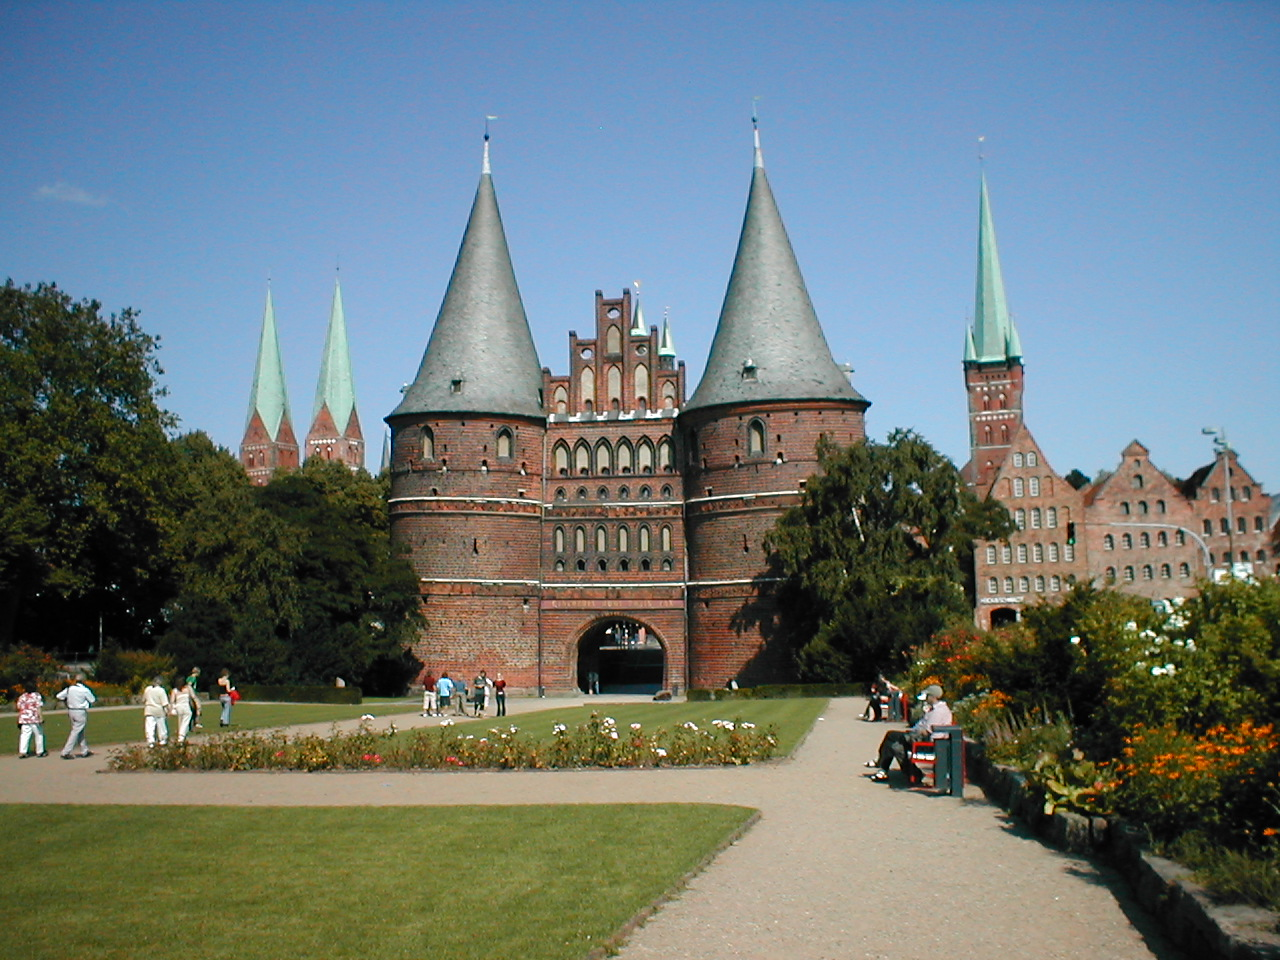
\includegraphics[width=0.75\textwidth]{images/LuebeckHolstentor}
		\caption[Kurzfassung für Abbildungsverzeichnis]{Ausführlicher Titel}
		\label{fig:Holstentor}
		\end{center}
\end{figure}

%Cref ergänzt automatisch Abbildung oder Tabellle etc.
In \Cref{fig:Holstentor} sehen wir das \todo{Eine Randnotiz!} Lübecker Holstentor.

\subsection{Tabelle}

\begin{table}
\centering
\footnotesize
\caption[Kurze Tabellenüberschrift]{Lange Tabellenüberschrift}
\label{tab:eins}
\begin{tabular}{p{1.4cm} p{2.0cm} p{2.0cm}}\toprule
			& A 			& B 		\\[0.1cm]\midrule
	1		& w				& s 		\\[0.2cm]
	2 		& e				& f			\\[0.2cm]
	3		& r				& s			\\[0.2cm]
	4 		& t				& n 		\\\bottomrule
\end{tabular}
\end{table}

In \Cref{tab:eins} sehen wir...

\subsection{Gleichung}

\begin{equation}\label{eq:test}
  a=b
\end{equation}

In \Cref{eq:test} sehen wir...

\subsection{Code-Listing}

\lstinputlisting[label={lst:hello}, caption={This is a code.}]{helloworld.cpp}


In \Cref{lst:hello} wird...

\subsection{Zitat}

Ein Zitat aus der Wikipedia:

\begin{quote}
	\begin{myquote}
		Die Universität zu Lübeck ist eine Hochschule in der Hansestadt Lübeck (Deutschland), die 1964 zunächst als zweite Medizinische Fakultät der Universität Kiel eingerichtet wurde. Studienangebot und Forschungstätigkeit der Universität zu Lübeck haben ihren Ausgangspunkt in der Medizin.
		\label{quote:uni}
	\end{myquote}
\end{quote}

\todo[inline,color=green!40,caption={Kurzversion des Todos}]{Ein Inline-Todo}

%
% Hinweis: CRef funktioniert nicht für Zitate! Bitte \quoteref{...} verwenden
%
In \quoteref{uni}...

\todo[inline]{Mit Besitzer und Datum}

\newpage

Etwas mehr Inhalt auf einer weiteren Seite

\newpage

Etwas mehr Inhalt auf noch einer tollen Seite



%---------------------------------------------------------------------------
% Noch mehr inhaltliche Chapter
%---------------------------------------------------------------------------


%---------------------------------------------------------------------------
% Anhang
%---------------------------------------------------------------------------
	\cleardoublepage
	\newpage
	\pagenumbering{roman}
	\setcounter{page}{1}
	\appendix

				\listoffigures

	    \listoftables

		

	%---------------------------------------------------------------------------

    %using: \abk{Abk.}{Abkürzung}
		\printnomenclature

		\printbibliography

    \printindex

\end{document}
